By nature, a random number generator (RNG) is a sequential algorithm,
as described in Figure~\ref{fig:rng1} below. Indeed, we shall describe a RNG
by its updating function $f$ changing deterministically the internal
state.  Each time the user requires a new realization of the uniform
distribution over $[0;1)$, the algorithm derives a value $u_k$ from
the current internal state $i_k$ and then updates this state with $f$.
Hence a first and important issue for parallel Monte Carlo
computations is to design independent RNGs that might run in parallel
while minimizing the communications between processors. It is quite
standard to use as many RNGs as computing cores in the computer or in
the cluster of computers. 


\begin{figure}[htb]
\centering \it
\begin{minipage}[c]{.6\linewidth}
  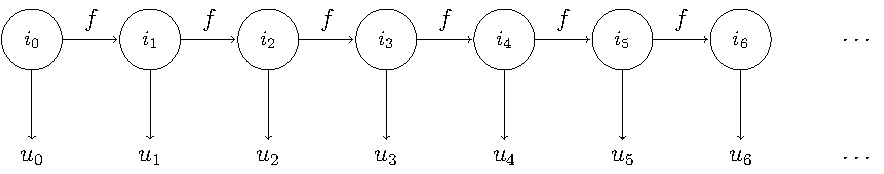
\includegraphics[width=\textwidth]{DCMT_rng.pdf}
  \caption[width=.6\textwidth]{\label{fig:rng1} \it\footnotesize
    \textbf{Random Number Generator.} A RNG is an algorithm
    that produces a sequence
    of floating numbers, says $u_0, u_1, \ldots$, that resembles a
    sequence of independant random numbers, uniformly distributed over
    $[0;1)$.
    It uses a sequence of
    internal states, say $i_0, i_1,\ldots$, which are computed by
    reccurence, namely, $i_{k+1}=f(i_k)$. The first internal state
    $i_0$ is often named the seed.}
\end{minipage}
\end{figure}

The second
version of DIYABC uses the Dynamic Creator (DCMT) of
\citet{DCMT} to look for a set of independent
Mersenne-Twister generators. Actually, the updating function $f$ of a
Mersenne-Twister generator is parametrized by a few integer
numbers. 
The output of the DCMT is a set of $N$ updating functions,
say $\{f^{(1)}, \ldots, f^{(N)}\}$, producing independent streams. 
That is, the $n$-th RNG is a sequence of iternal states
$i_0^{(n)},i_1^{(n)}, i_2^{(n)}, \ldots$ satisfying
$i_{k+1}^{(n)}=f^{(n)}(i_k^{(n)})$
that gives rise to a sequence of independent, uniformly distributed numbers
$u_0^{(n)}, u_1^{(n)}, u_2^{(n)},\ldots$.
We found that the DCMT was simple to use and gave good results.  There
is no limitation on the number $N$ of RNGs it produces. Once initialized,
the different RNGs do not require any communication between them and
each of them runs as quickly as a single Mersenne-Twister
generator. But an important limitation is that it is impossible to add a
new RNG to the set produced by the DCMT. Practically, this means that
we have to know \textit{a priori} a bound on the number of
jobs working together in parallel. See XXX Alex XXX.





%%% Local Variables: 
%%% mode: latex
%%% TeX-master: "Notice_DIYABC_principal"
%%% End: 
